\documentclass[9pt]{extarticle}

\usepackage[utf8]{inputenc}
\usepackage[english]{babel}
\usepackage{hyperref}
\usepackage{extsizes}
\usepackage{caption}
\usepackage[table]{xcolor}
\definecolor{lgray}{gray}{0.95}

\usepackage[square,numbers]{natbib}
\bibliographystyle{plainnat}
\setcitestyle{authoryear,open={(},close={)}}

\usepackage{amsfonts, amsmath, amssymb, amsthm}

\newtheorem{theorem}{Theorem}[section]

\usepackage{graphicx}
\usepackage{float}

\usepackage[margin=1in]{geometry}

\usepackage[utf8]{inputenc}
\usepackage{fancyhdr}
 
\pagestyle{fancy}
\fancyhf{}

\rhead{Benjamin Cox}
\chead{Statistical Consultancy -- Assessment 1}
\lhead{Due 6th November}
\cfoot{Page \thepage}

\begin{document}

\section{Introduction}

We consider data on the gas consumption of dwellings of various types throughout North-East England. We have data on the gas consumption, age of the property, type of property, floor area of property, depth of loft insulation, whether cavity wall insulation is fitted, and whether a new boiler has been installed.

All but the gas consumption data is categorical, meaning that for example we do not know the precise age of the property but rather that it lies in a range of ages. This will impact our analysis and make it somewhat less accurate, but is a common trade-off, as it is easier to collect and store data of this sort. Obviously the type of property must be categorical, for example. We must note that the gas consumption has been somewhat severely rounded, leading to it, although truly continuous, having some properties (and difficulties) of a categorical variable. We will handle it as continuous, although we must keep the rounding in mind.

We will note that the gas consumption has been pre-corrected for weather, so this will not be a factor in our analysis. The data has also been selected to be representative of the housing stock, which will allow for us to draw more general conclusions. All of the properties use gas as the main mode of heating. When we refer to a `unit' of gas we mean 1 kWh per year.

\section{Statistical Analysis}

\subsection{Handling the Missing Data}

First we must check the data for missing values and decide how to continue. An aggregate plot of the data is found in Figure \ref{fig:aggrmiss}. Obviously one must think about the ramifications of this, but we can clearly see that a large proportion of the data for boilers is missing, making it somewhat less useful for our analysis. We assume a completely random missing data mechanism, as this is the most likely given the nature of our data. This means that using predictive mean matching should give us results that are unbiased. We will use this going forward.

Another way of dealing with missingness in categorical variables is to make NA a category. This is not what we are going to use, but it is a simple way of getting the analysis to work.

We use the R package \texttt{mice} to perform multiple imputation on our data to obtain a full dataset. We will carefully consider the differences between our complete case analysis and our analysis of the imputed data and attempt to explain any discrepancies. The implementation of predictive mean matching that is used selects randomly from the 5 nearest neighbours, so we fix our random seed to get repeatable results.

\subsection{Initial Analysis}

There are a few factors that we will account for. The first is that houses are not lines, but (nearly) cubes. We must consider that a house loses heat primarily through its four enclosing walls and its roof. One could think that a four fold increase in gas consumption would be needed to heat a house that is twice larger in length and depth. This means that it would be appropriate to use a square-root transformation on the gas consumption. We must be careful to acknowledge that the age and floor area, although inputted as numerical, are treated as factors. To do otherwise would invalidate the analysis.

The decision to use the square root is validated by looking at the quantile-quantile plots in Figure \ref{fig:qqplots}. We see that the de-trended plot for the transformed response variable gives us far superior results. We will continue with our analysis using the transformed response. Wee see that our data is heavily tailed. It has a very severe right tail which we ameliorate by taking the square root. This is due to the rounding of values creating large instantaneous increases in density, which violate normality. Hence much of our analysis will be of `root units', which we square to get back our initial units of kWh.

Looking at the data given in Figure \ref{fig:datavis} we see that the median gas consumption is 13000 units. 

\subsection{Model Comparison and Selection}
To generate the full model we must first look at the independence of terms in the data. We do this using the $\chi^2$ test, the results of which are given in Table \ref{tab:chi}. We see that many of the variables are interdependent, which will influence our results. We see that the age, type, and floor area of a property are highly related, which is what we realistically expected. We regress the square root of the gas consumption on all of the predictor variables to obtain our full model. The diagnostic plots are given in Figure \ref{fig:fmdiag}. These plots are perfectly sufficient, the leverages are low so our model is quite stable. 

We will now compare the full model to two sub-models. The sub-models regress gas consumption on the base property (age, type, floor area) and on modifications to the property (loft insulation, cavity wall insulation, new boiler) respectively. The diagnostic plots are given in Figure \ref{fig:smdiag}. The diagnostic plots show that both are valid models which give similar results to the initial model. We compare them to the initial model using an ANOVA test. We see that the modifications model is significantly different from the initial model, so the base properties of the property have significant effects. The property model is not different at the five percent level, so we fail to reject the hypothesis that both the property model and the full model explain the data adequately. We compare the residual sum of squares and see that the full model has an RSS of 1244518, the property model has an RSS of 1248346, and that the modification model has an RSS of 1880124. We see that the modifications to the property have a significantly lesser effect on the consumption than the property properties.

We choose to use the full model for our analysis as we wish to see the effects of the modifications on the property, as these are measures that can be taken after a property is constructed. The regression coefficients are given in Table \ref{tab:fulmo}.

\section{Discussion of Results}

We are discussing the effect of the different variables on the square root of the gas consumption. The `base' results are for a Bungalow in age band 1, in floor area band 1, with loft insulation greater than 150mm, without cavity walls, and without a new boiler. The predicted square root of consumption for this property is 103.7. 

\subsection{Effect of Age}
We see that age has less of an effect than might be expected. The first four age bands have minimal effect. The fifth and the sixth age bands have more significant differences, with a decrease on average of 7.84 and 13.76 respectively. This means that new builds have decreased gas consumption. This may be due to the types of property built in new builds, as in \ref{tab:chi} we see that they are not independent.

\subsection{Effect of Type}
We see that the type of property is very significant in determining the gas consumption. Detached houses have an increased root gas consumption compared to bungalows, consuming 12.7 root units more. Semi detached consume only very slightly more, to the point that it is not significant (it is less than the standard error of the estimate). Terraced and end of terrace houses consume less. Flats consume significantly less, with 22.9 less root units on average, corresponding to 525 units less on average. 

\subsection{Effect of Floor Area}
We see that floor area has a significant effect on the gas consumption. All of them are significantly different from each other. The largest floor area consumes on average 52.56 root units, or 2762 units on average more than the smallest floor area. This is also not independent of the type of property, so we must know that changing one should have an effect on the other (ie a property with a large floor area is less likely to be a flat than detached).

\subsection{Effects of Modifications to The Property}
These effects are smaller, so will be discussed in conjunction. First we note that we see in Table \ref{tab:chi} that all of the modifications are largely independent of each other. This meshes with what we expect. We see that a new boiler decreases root gas consumption by 2.78, corresponding to an average decrease in consumption of 7.71 units. Adding cavity wall insulation has no appreciable average effect on gas consumption. Adding loft insulation above 150mm decreases root gas consumption on average by 1.98 units, corresponding to an average decrease of 3.90 units of gas consumption. 


\section{Conclusions}

%\bibliography{references}

\appendix

\section{Plots and Figures}

\begin{figure}[H]
	\centering
	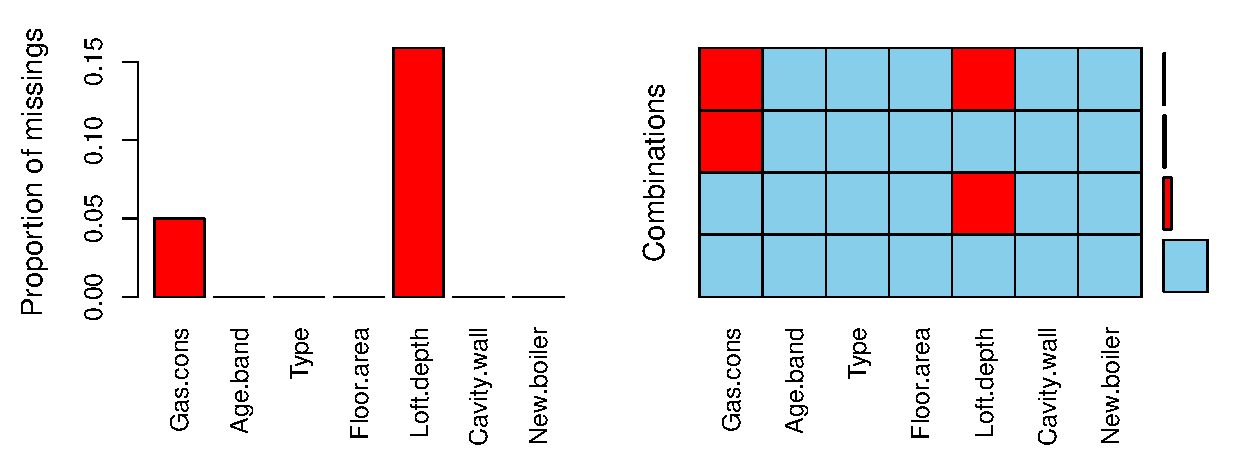
\includegraphics[width=0.7\textwidth]{aggr_missplot}
	\caption{Aggregate plot of missingness in our data}
	\label{fig:aggrmiss}
\end{figure}

\begin{figure}[H]
	\centering
	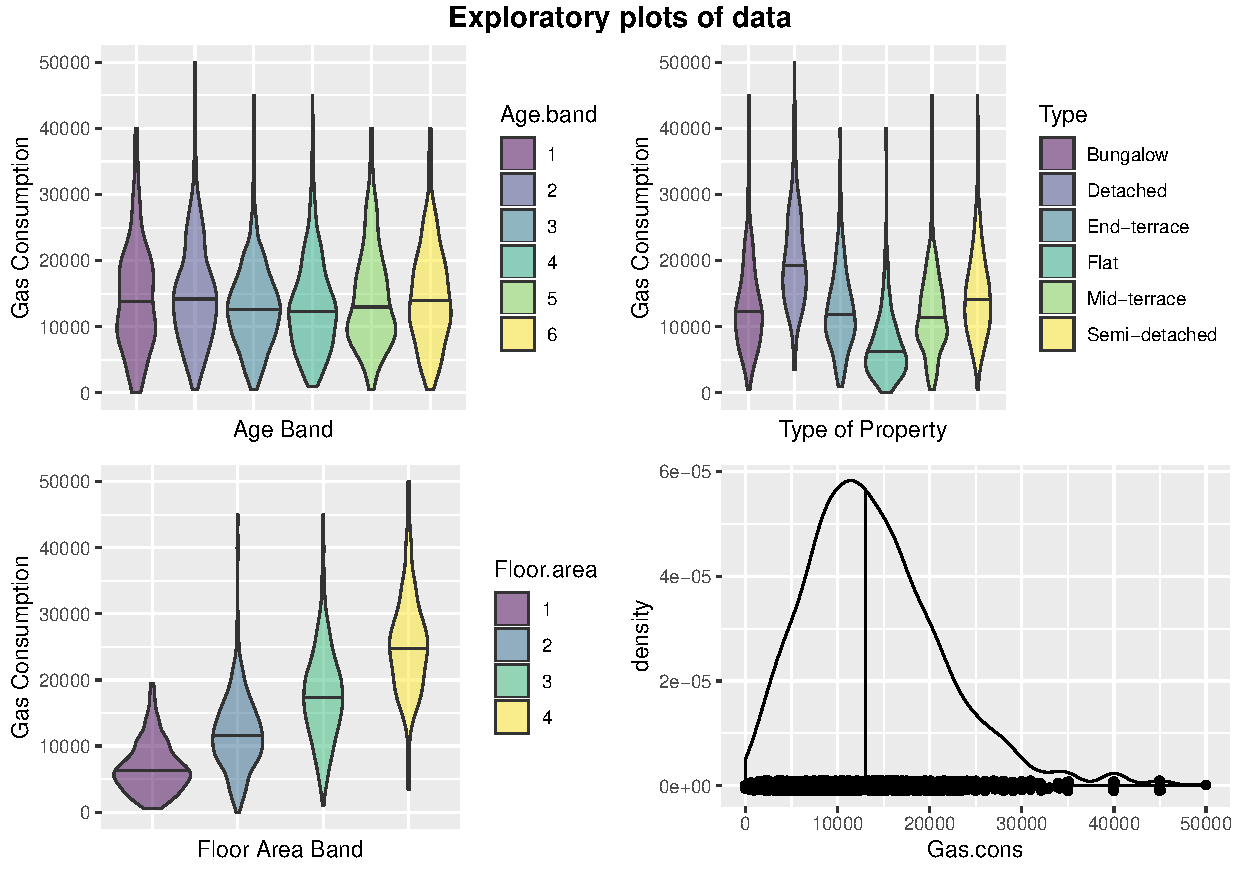
\includegraphics[width=0.7\textwidth]{datavis}
	\caption{Visualisation of data relating to gas consumption}
	\label{fig:datavis}
\end{figure}


\begin{figure}[H]
	\centering
	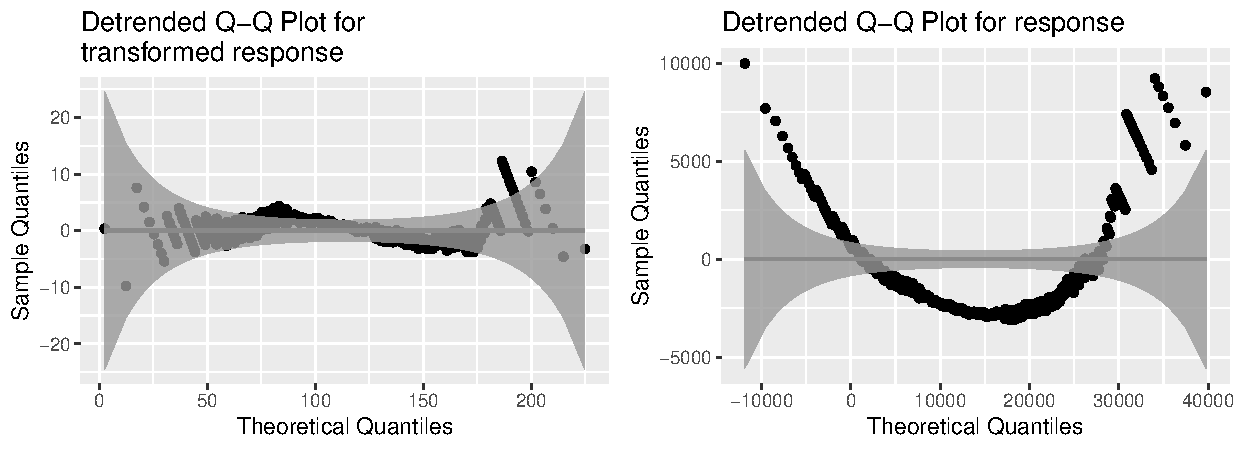
\includegraphics[width=0.7\textwidth]{qqplots}
	\caption{Model Q-Q plots for the transformed and non-transformed models}
	\label{fig:qqplots}
\end{figure}

\begin{figure}[H]
	\centering
	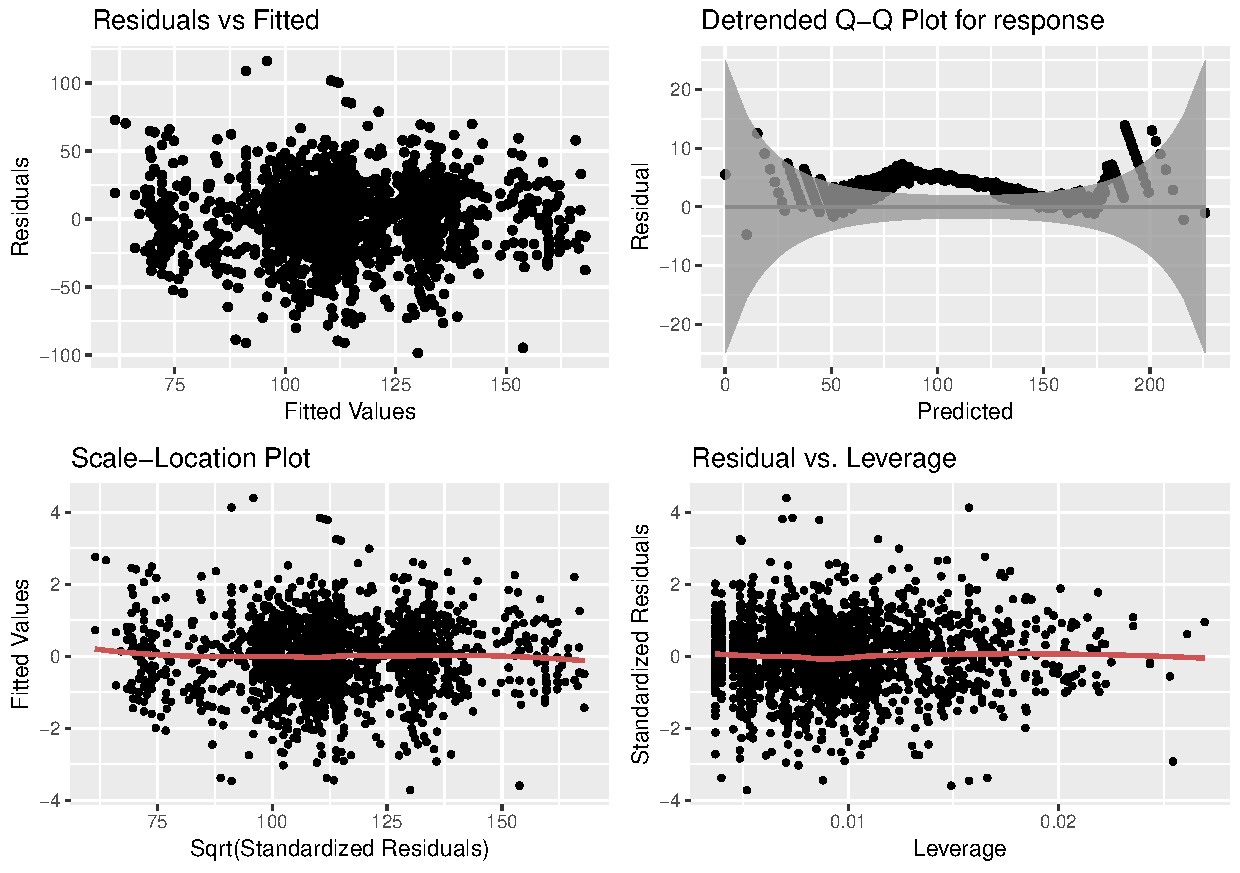
\includegraphics[width=0.7\textwidth]{fm_diag}
	\caption{Model diagnostic plots for our full model}
	\label{fig:fmdiag}
\end{figure}

\begin{figure}[H]
	\centering
	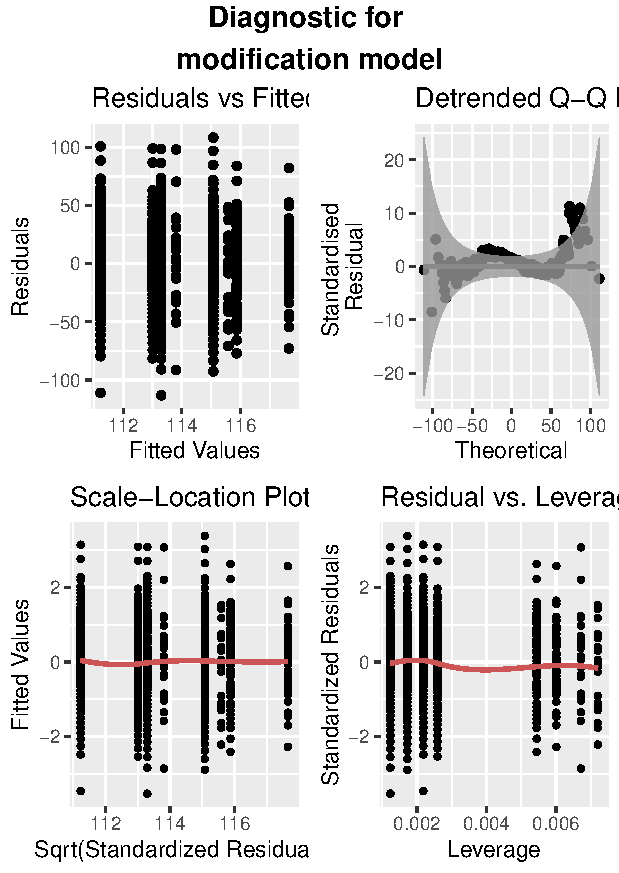
\includegraphics[width=0.4\textwidth]{diag_modif}
	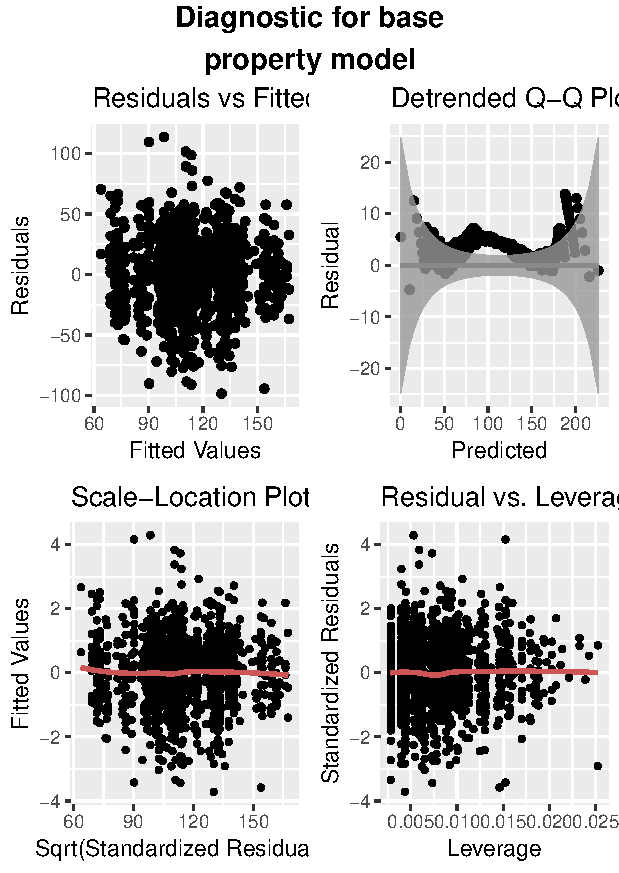
\includegraphics[width=0.4\textwidth]{diag_prop}
	\caption{Model diagnostic plots for our sub-models}
	\label{fig:smdiag}
\end{figure}

\section{Tables}

\begin{table}[H]
	\centering
	\rowcolors{1}{white}{lgray}
	\begin{tabular}{r|llr}
		\hline
		& Row & Column & p.value \\ 
		\hline
		1 & Gas.cons & Age.band & 0.03 \\ 
		2 & Gas.cons & Type & 0.00 \\ 
		3 & Gas.cons & Floor.area & 0.00 \\ 
		4 & Gas.cons & Loft.depth & 0.55 \\ 
		5 & Gas.cons & Cavity.wall & 0.12 \\ 
		6 & Gas.cons & New.boiler & 0.31 \\ 
		7 & Age.band & Type & 0.00 \\ 
		8 & Age.band & Floor.area & 0.00 \\ 
		9 & Age.band & Loft.depth & 0.00 \\ 
		10 & Age.band & Cavity.wall & 0.00 \\ 
		11 & Age.band & New.boiler & 0.23 \\ 
		12 & Type & Floor.area & 0.00 \\ 
		13 & Type & Loft.depth & 0.72 \\ 
		14 & Type & Cavity.wall & 0.00 \\ 
		15 & Type & New.boiler & 0.16 \\ 
		16 & Floor.area & Loft.depth & 0.87 \\ 
		17 & Floor.area & Cavity.wall & 0.00 \\ 
		18 & Floor.area & New.boiler & 0.35 \\ 
		19 & Loft.depth & Cavity.wall & 0.68 \\ 
		20 & Loft.depth & New.boiler & 0.08 \\ 
		21 & Cavity.wall & New.boiler & 0.49 \\ 
		\hline
	\end{tabular}

\vspace{0.5em}
p.value less than 0.05 means variables are (likely to be) statistically dependent.
\caption{Table of results from Chi Squared test for independence. }
\label{tab:chi}
\end{table}

\begin{table}[H]
	\centering
	\rowcolors{1}{white}{lgray}
	\begin{tabular}{r|lrr}
		\hline
		& Term & Estimate & Standard Error \\ 
		\hline
		1 & (Intercept) & 103.68 & 4.06 \\ 
		2 & Age.band2 & -0.96 & 2.37 \\ 
		3 & Age.band3 & -3.58 & 2.27 \\ 
		4 & Age.band4 & -4.84 & 2.34 \\ 
		5 & Age.band5 & -7.85 & 2.87 \\ 
		6 & Age.band6 & -13.76 & 2.95 \\ 
		7 & TypeDetached & 12.66 & 2.88 \\ 
		8 & TypeEnd-terrace & -5.97 & 2.74 \\ 
		9 & TypeFlat & -22.92 & 3.11 \\ 
		10 & TypeMid-terrace & -11.70 & 2.33 \\ 
		11 & TypeSemi-detached & 0.75 & 2.08 \\ 
		12 & Floor.area2 & 11.38 & 3.31 \\ 
		13 & Floor.area3 & 30.27 & 3.62 \\ 
		14 & Floor.area4 & 52.56 & 4.56 \\ 
		15 & Loft.depthLe & 1.98 & 1.98 \\ 
		16 & Cavity.wallY & -0.09 & 1.31 \\ 
		17 & New.boilerY & -2.78 & 1.34 \\ 
		\hline
	\end{tabular}
\caption{Table of regression coefficients for the full model.}
\label{tab:fulmo}
\end{table}




\end{document}